\subsection{常用术语}
为方便理解,本设计中部分常见术语规定如下,具体设计中如有特殊术语或图例已在图中绘制图例,此处不再赘述。

\begin{description}
  \item [指向箭头] 全景漫游用于进行场景切换的箭头标识
\end{description}

\subsection{导航界面设计}
导航功能试图在单个界面里包容更多的上下文信息以便用户准确定位自身所在,同时通过多界面并存的形式方便用户可以随时查看早前访问过的页面。根据前文人的视域的特性,导航界面整体功能菜单向下布置,主要元素垂直方向布置,方便用户浏览。因全景漫游具有一定的空间感,将部分界面设计成多面环状排布更有利于用户查看相关信息。

导航漫游记录以 3D 界面形式呈现。用户可由当前界面观察到早先访问过的界面的一部分,有助于用户建立上下文感知。如图\ref{fig:d-03}。

\begin{figure}[htp]
\centering
\fbox{
  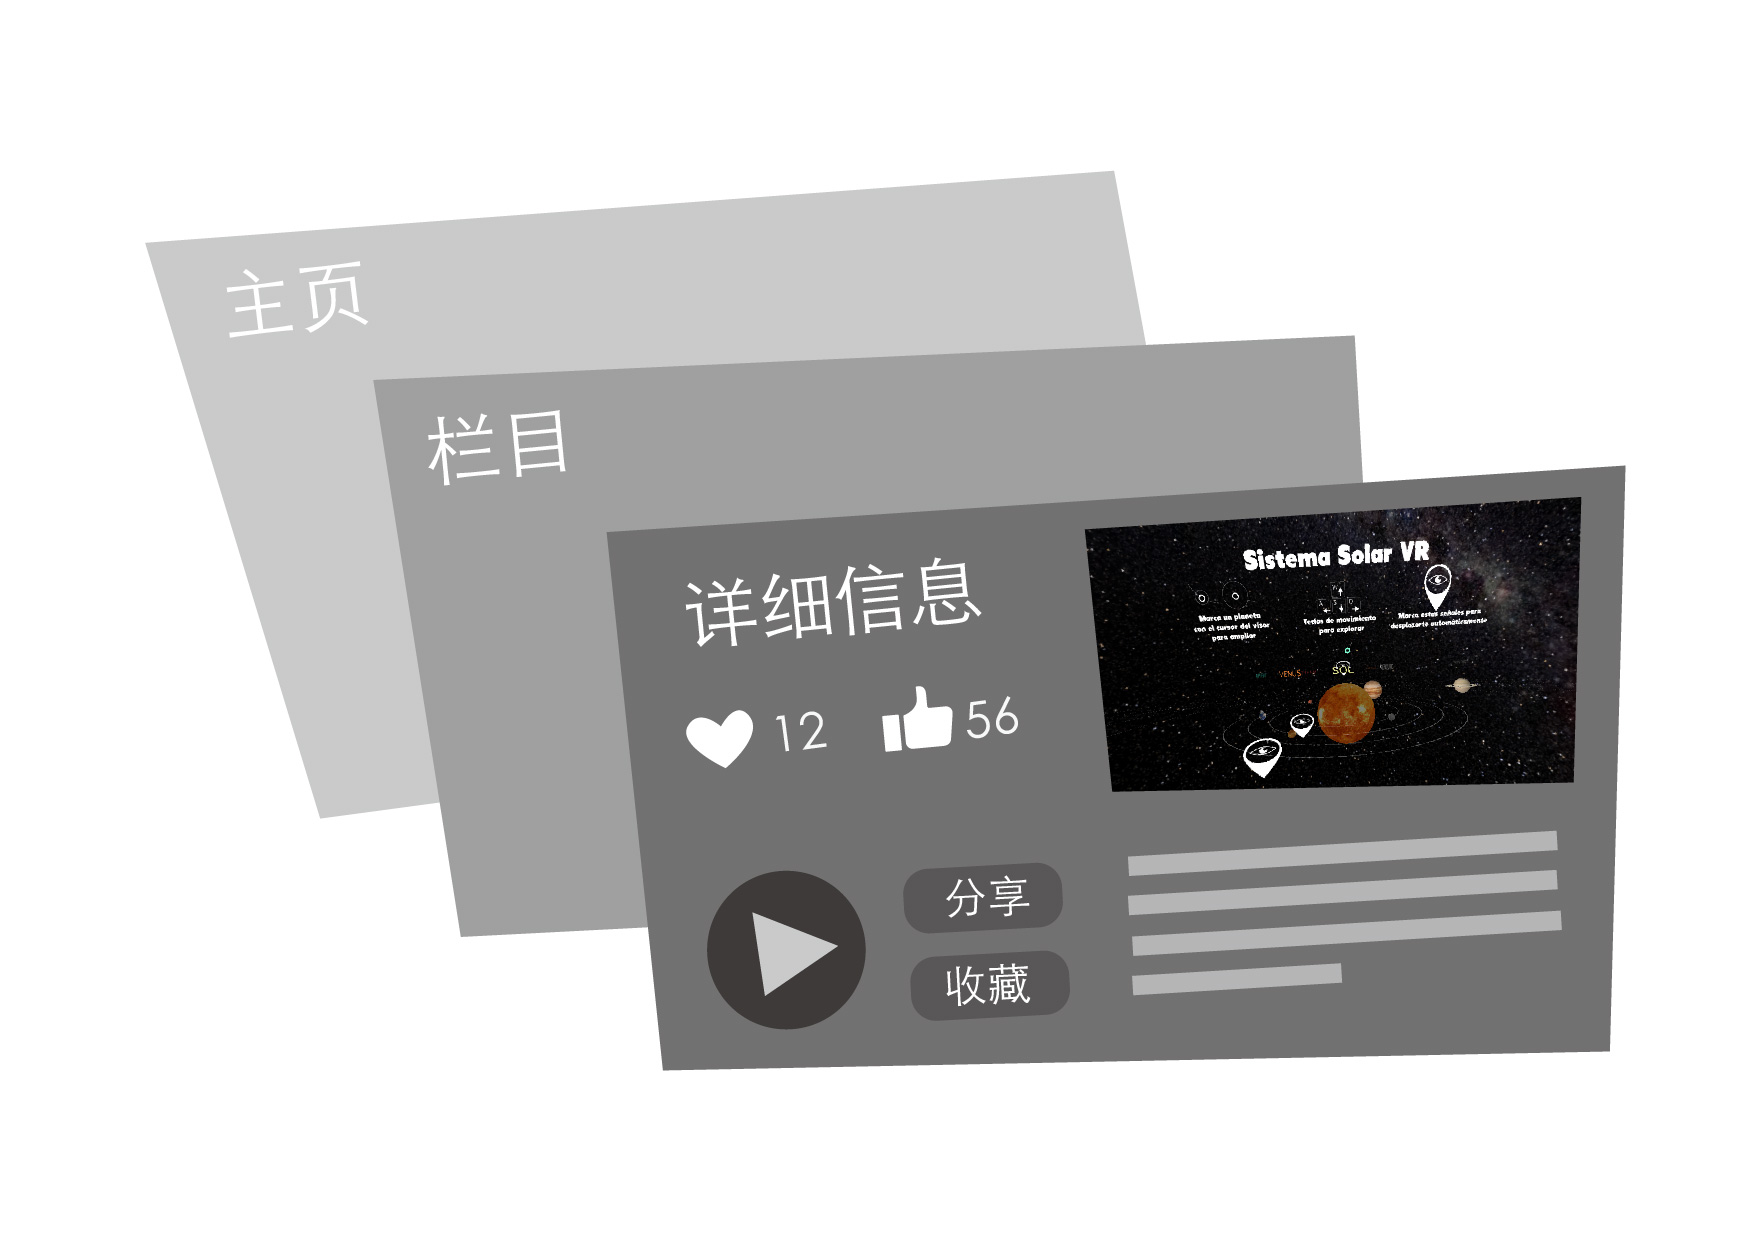
\includegraphics[width=.5\textwidth]{design/d-03}
}
\caption{3D界面}
\label{fig:d-03}
\end{figure}

\subsubsection{主界面}
主界面采用格式塔法则将各功能元素按区块设置。根据视觉特性,人的视觉注意是从左上至右上,再从左下至右下。中心界面左上为推荐模块,是用户进入界面后第一眼看到的场景,最容易吸引用户注意力。右上方为类别菜单,帮助用户建立漫游系统的分类体系。整个下方为二级推荐栏目,这里是系统根据用户特征及热门栏目综合计算得出的推荐项目。

左侧界面为部分置顶的类别界面,下方为标签栏,提供给用户切换分类的功能,用户可以通过浏览上部菜单了解到该类别部分场景的信息。右侧界面为历史记录或收藏夹界面。

主界面设计如图\ref{fig:d-01}。

\begin{figure}[htp]
\centering
\fbox{
  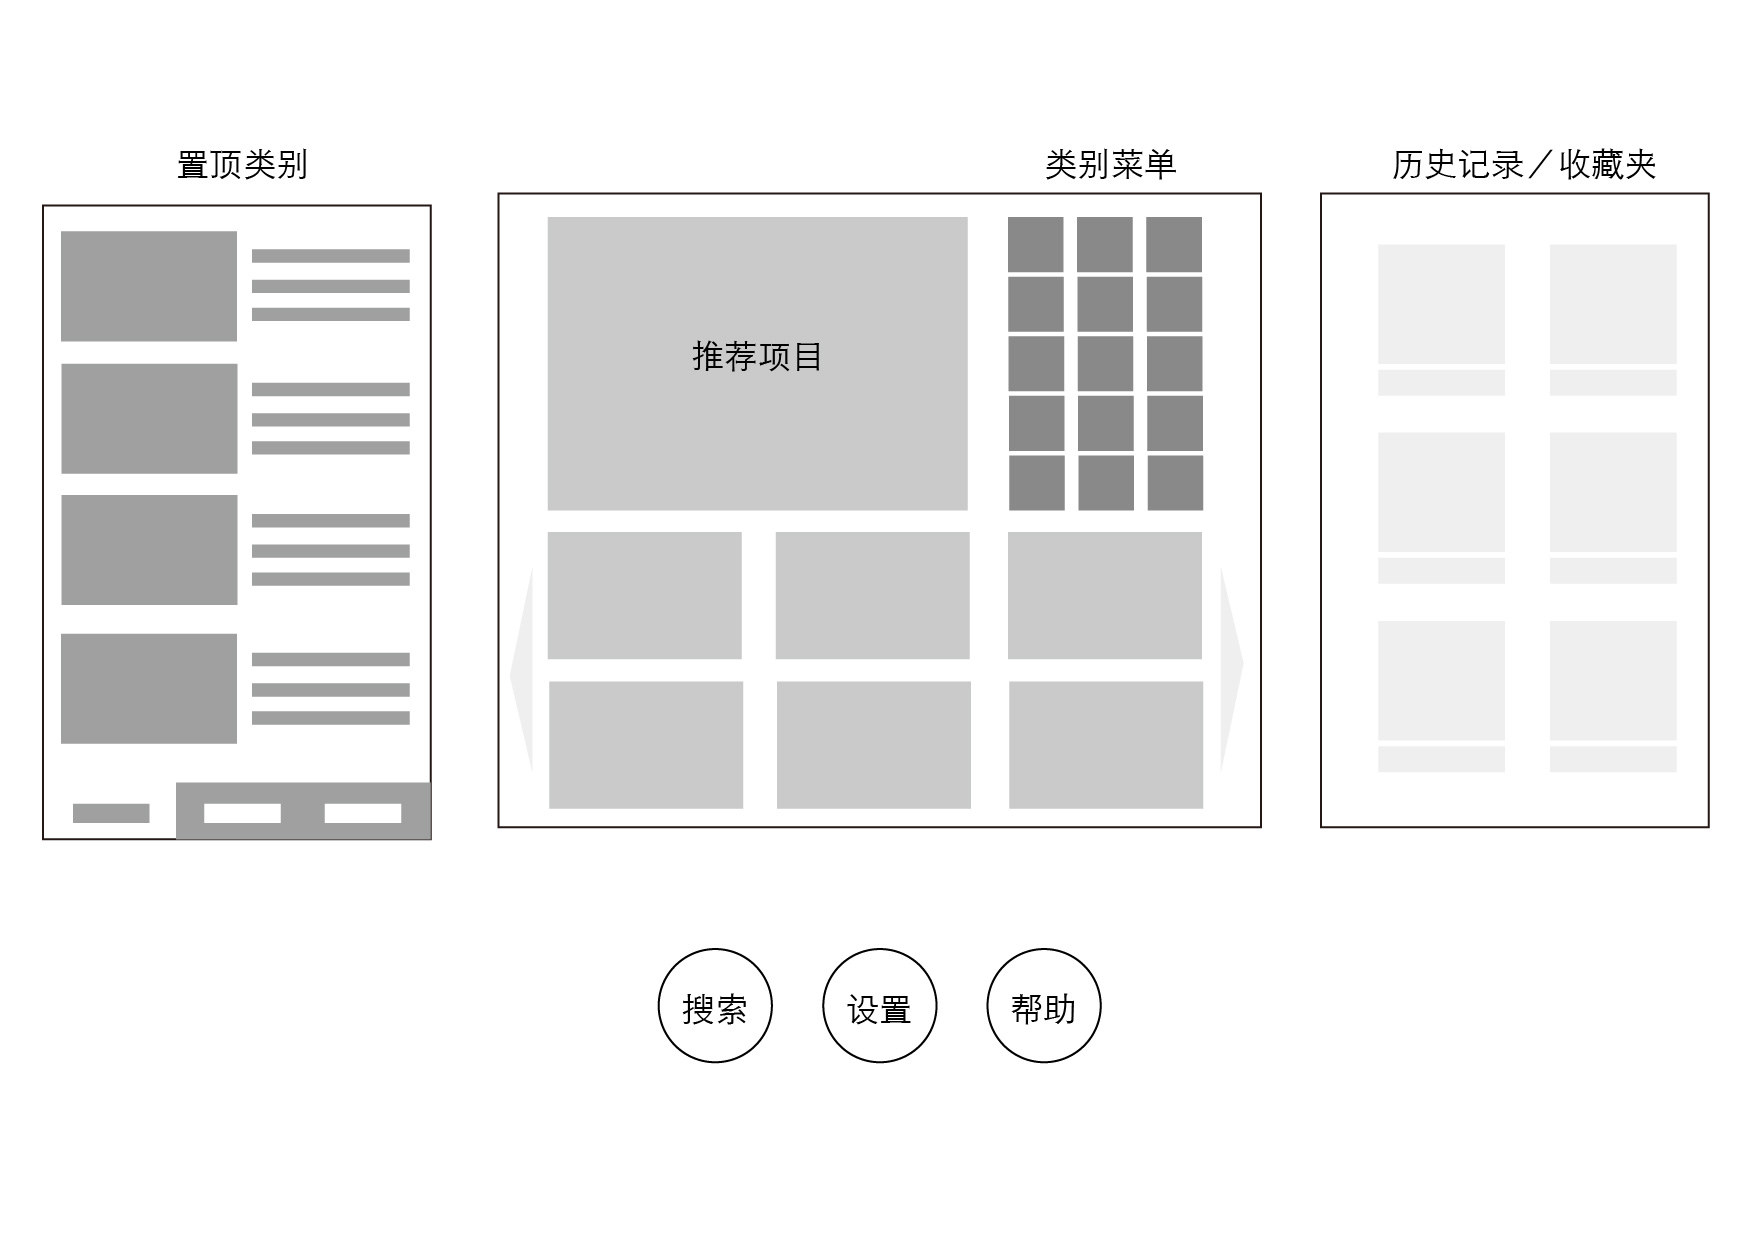
\includegraphics[width=.5\textwidth]{design/d-01}
}
\caption{主界面}
\label{fig:d-01}
\end{figure}

\subsubsection{类别界面}
类别界面则提供了更多分类以供选择,同时通过分页形式展示了全部的分类项目,考虑到用户操作次数的限制,通过筛选器查找分类里某个场景应用的功能意义较小,故在此只设计出以分类名查看场景应用的形式。分类的换页是不常用的功能,用户浏览的顺序大多为按类别查看第一页的项目,所以把分页设置于右侧,并且分页切换是上下排布,更利于用户通过仰头低头进行切换,降低了使用负担。类别界面如图\ref{fig:d-06}。

\begin{figure}[htp]
\centering
\fbox{
  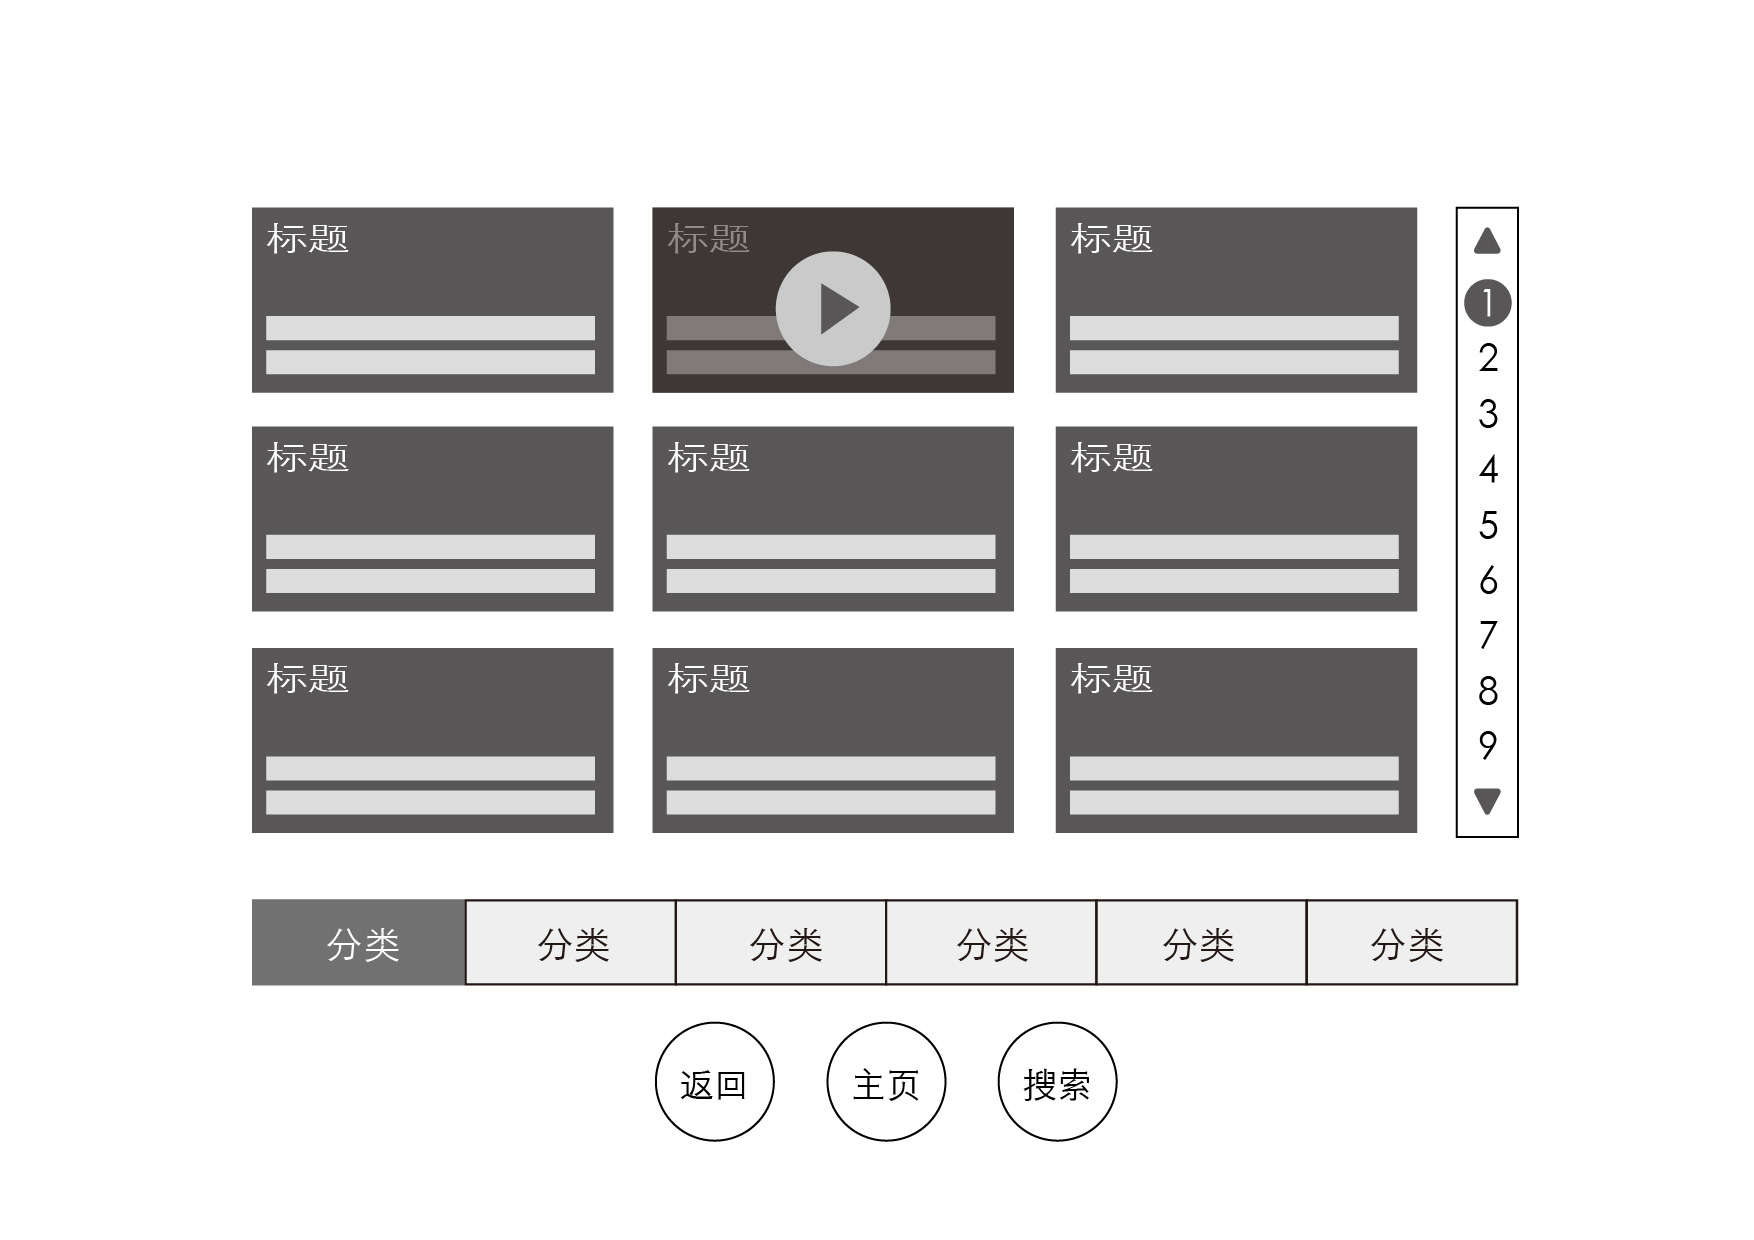
\includegraphics[width=.5\textwidth]{design/d-06}
}
\caption{类别界面}
\label{fig:d-06}
\end{figure}

考虑到存在用户偏向物理存在感强的菜单界面,故也有仿星系运动的界面如图\ref{fig:d-02}。这种界面趣味性更强,但因其与常见二维界面差别过大,开发难度和实现上均有难度,故本文只做示例,下文仍以平面导航界面为例说明。

\begin{figure}[htp]
\centering
\fbox{
  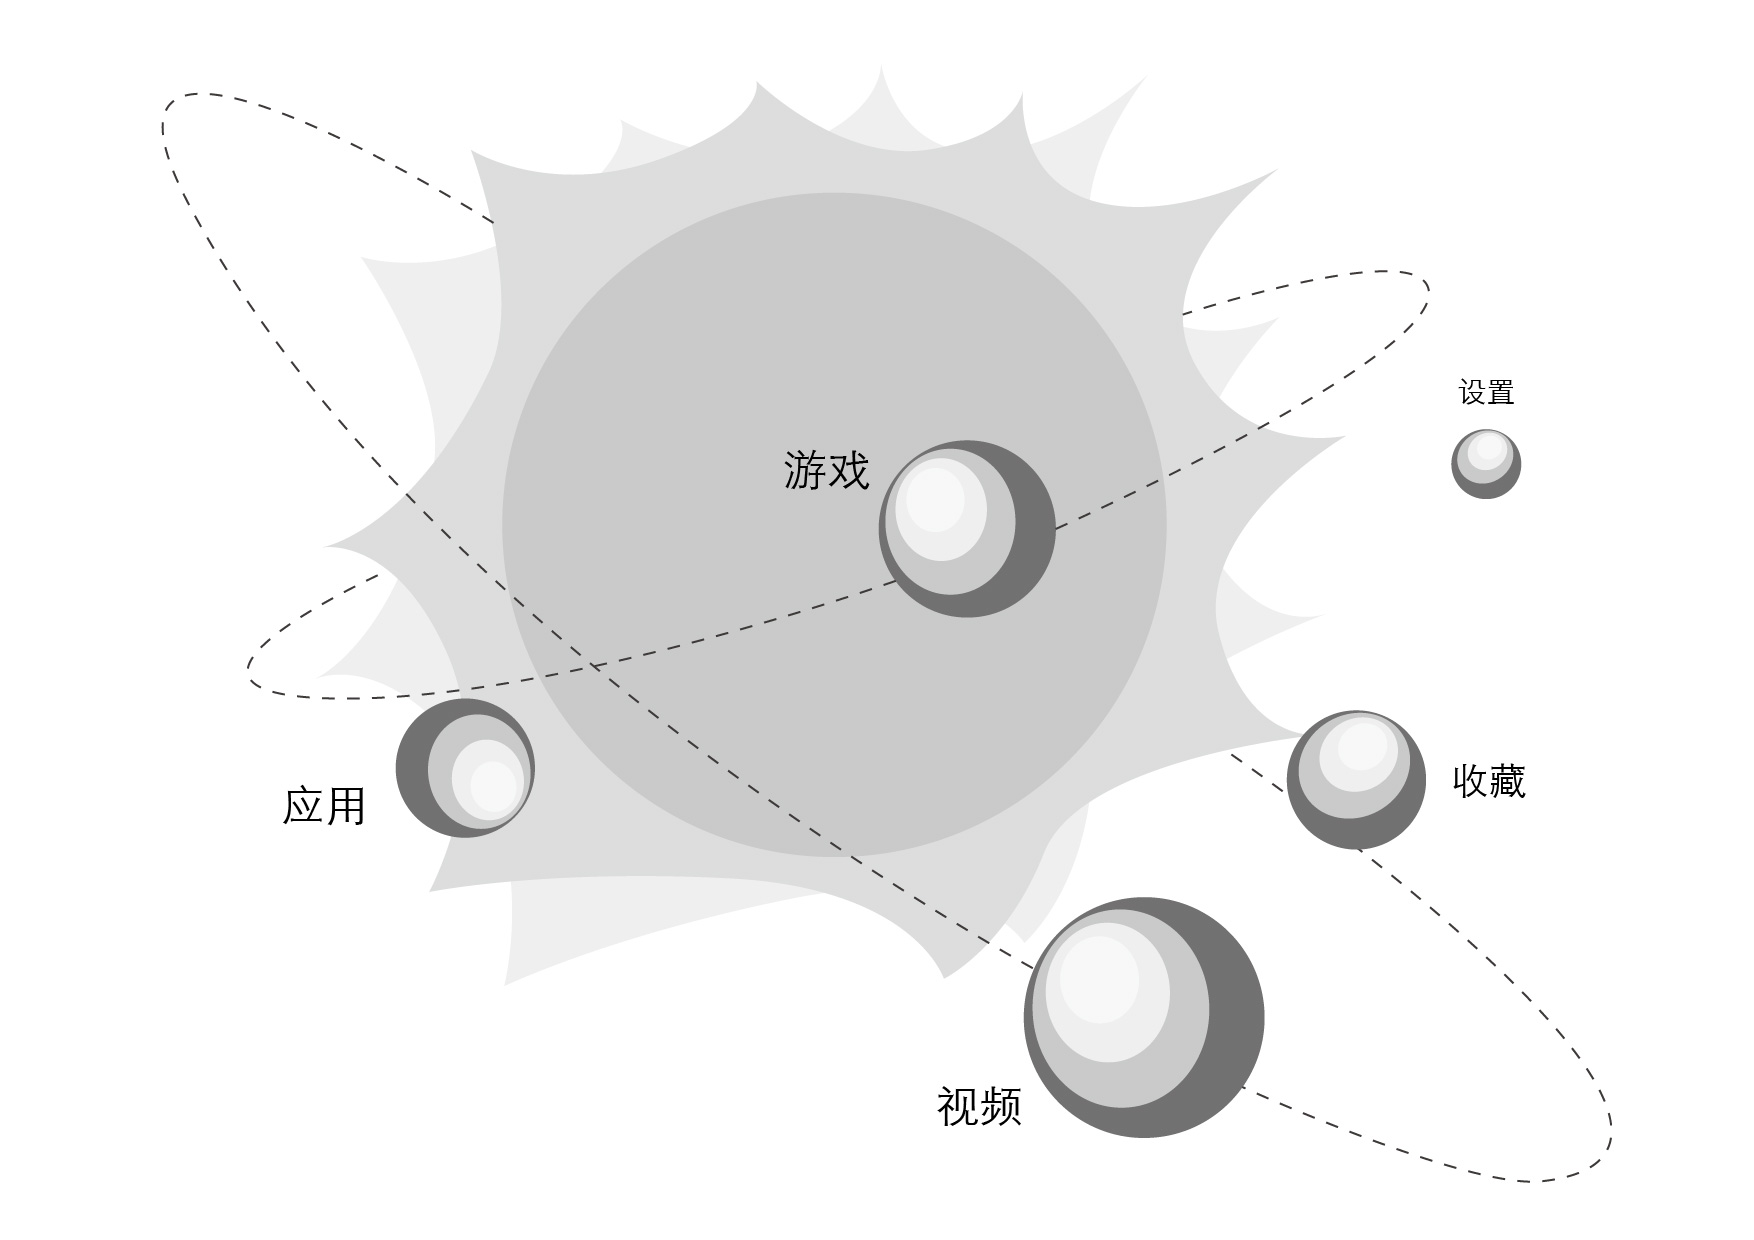
\includegraphics[width=.5\textwidth]{design/d-02}
}
\caption{星系状界面}
\label{fig:d-02}
\end{figure}

\subsubsection{详情界面}

单个场景详情界面如图\ref{fig:d-07}。

\begin{figure}[htp]
\centering
\fbox{
  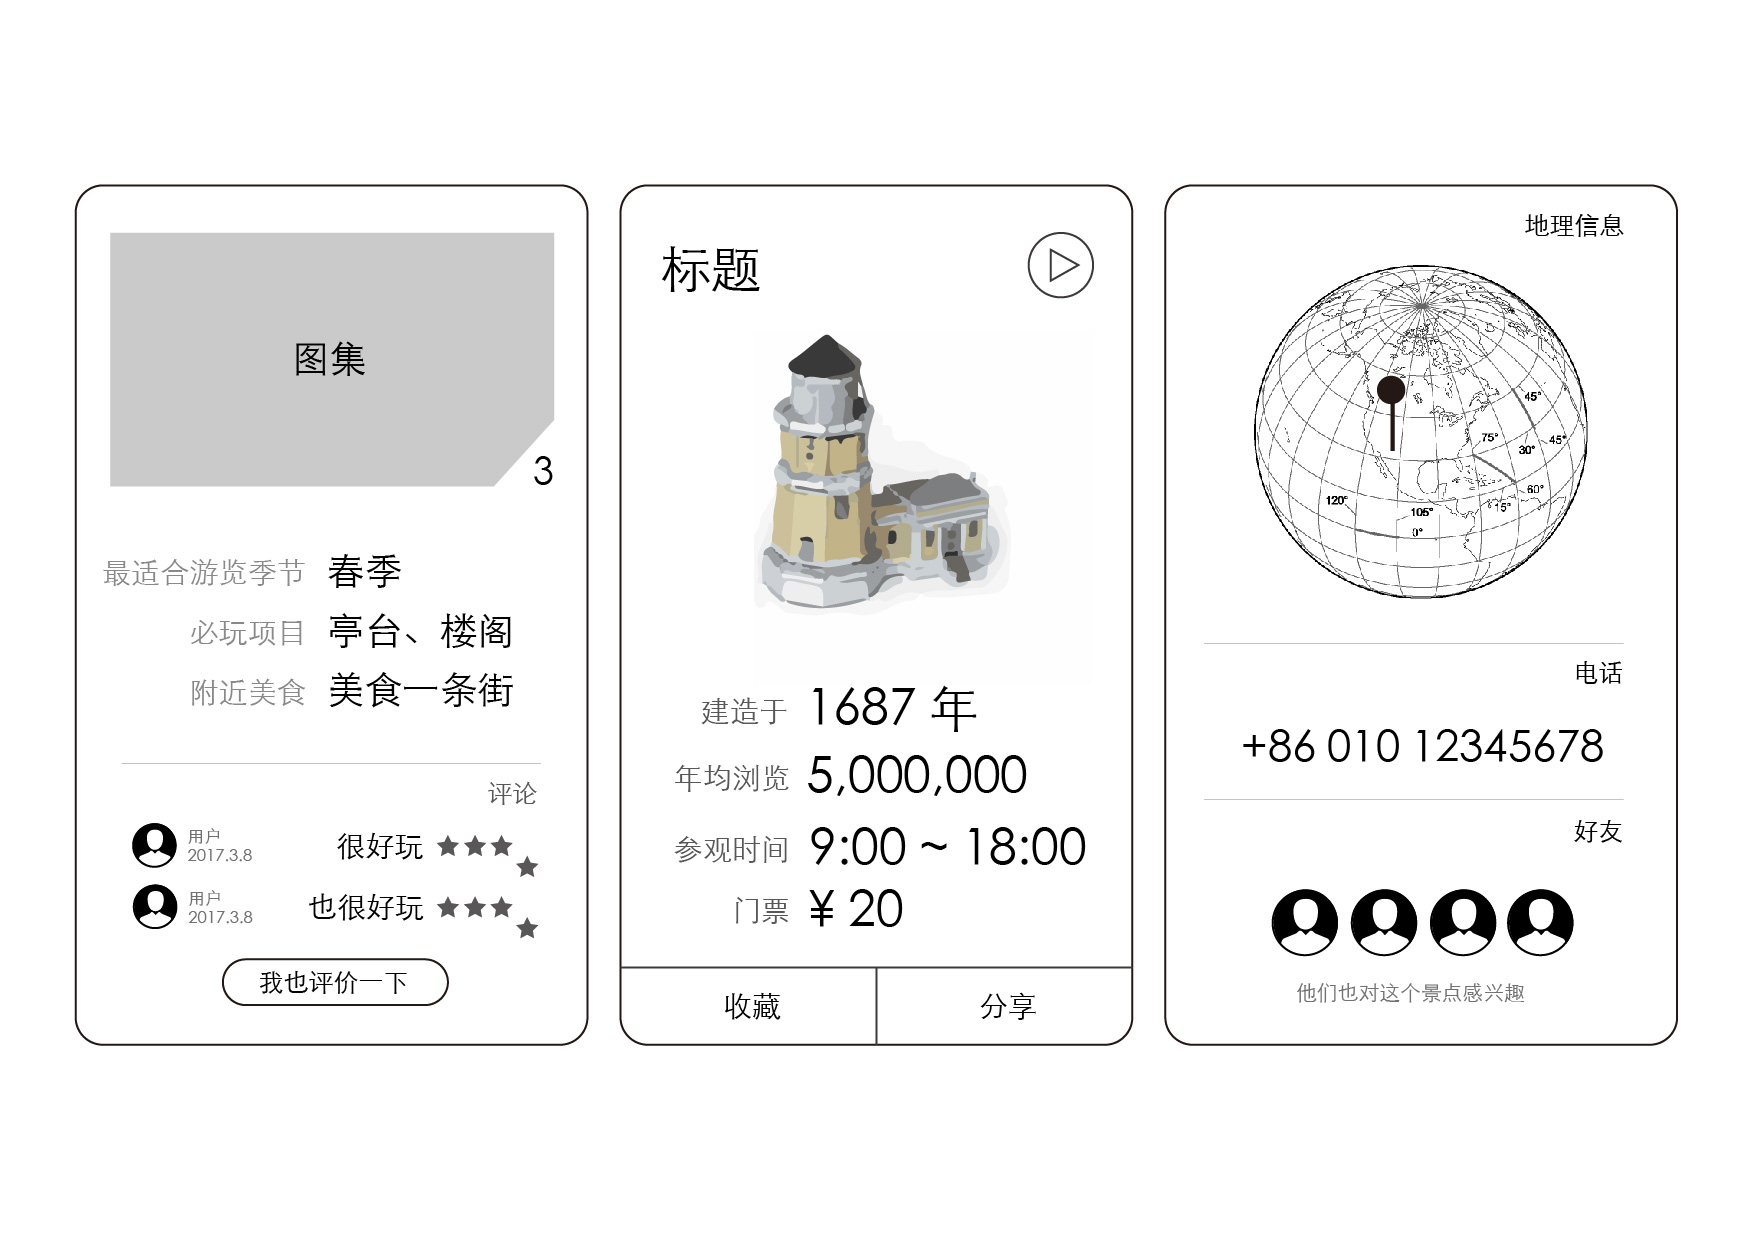
\includegraphics[width=.5\textwidth]{design/d-07}
}
\caption{单个场景详情界面}
\label{fig:d-07}
\end{figure}

\subsection{漫游界面设计}
\begin{itemize}
	\item 漫游界面带有紧急退出区域,只需注视 1~2 秒以上就可以紧急退出场景,避免眩晕加重。
	\item 可通过地面上的指示图标切换场景。
	\item 可通过场景中的热点区域查看详细信息。
\end{itemize}
如图\ref{fig:scenery}。

\begin{figure}[htp]
\centering
\fbox{
  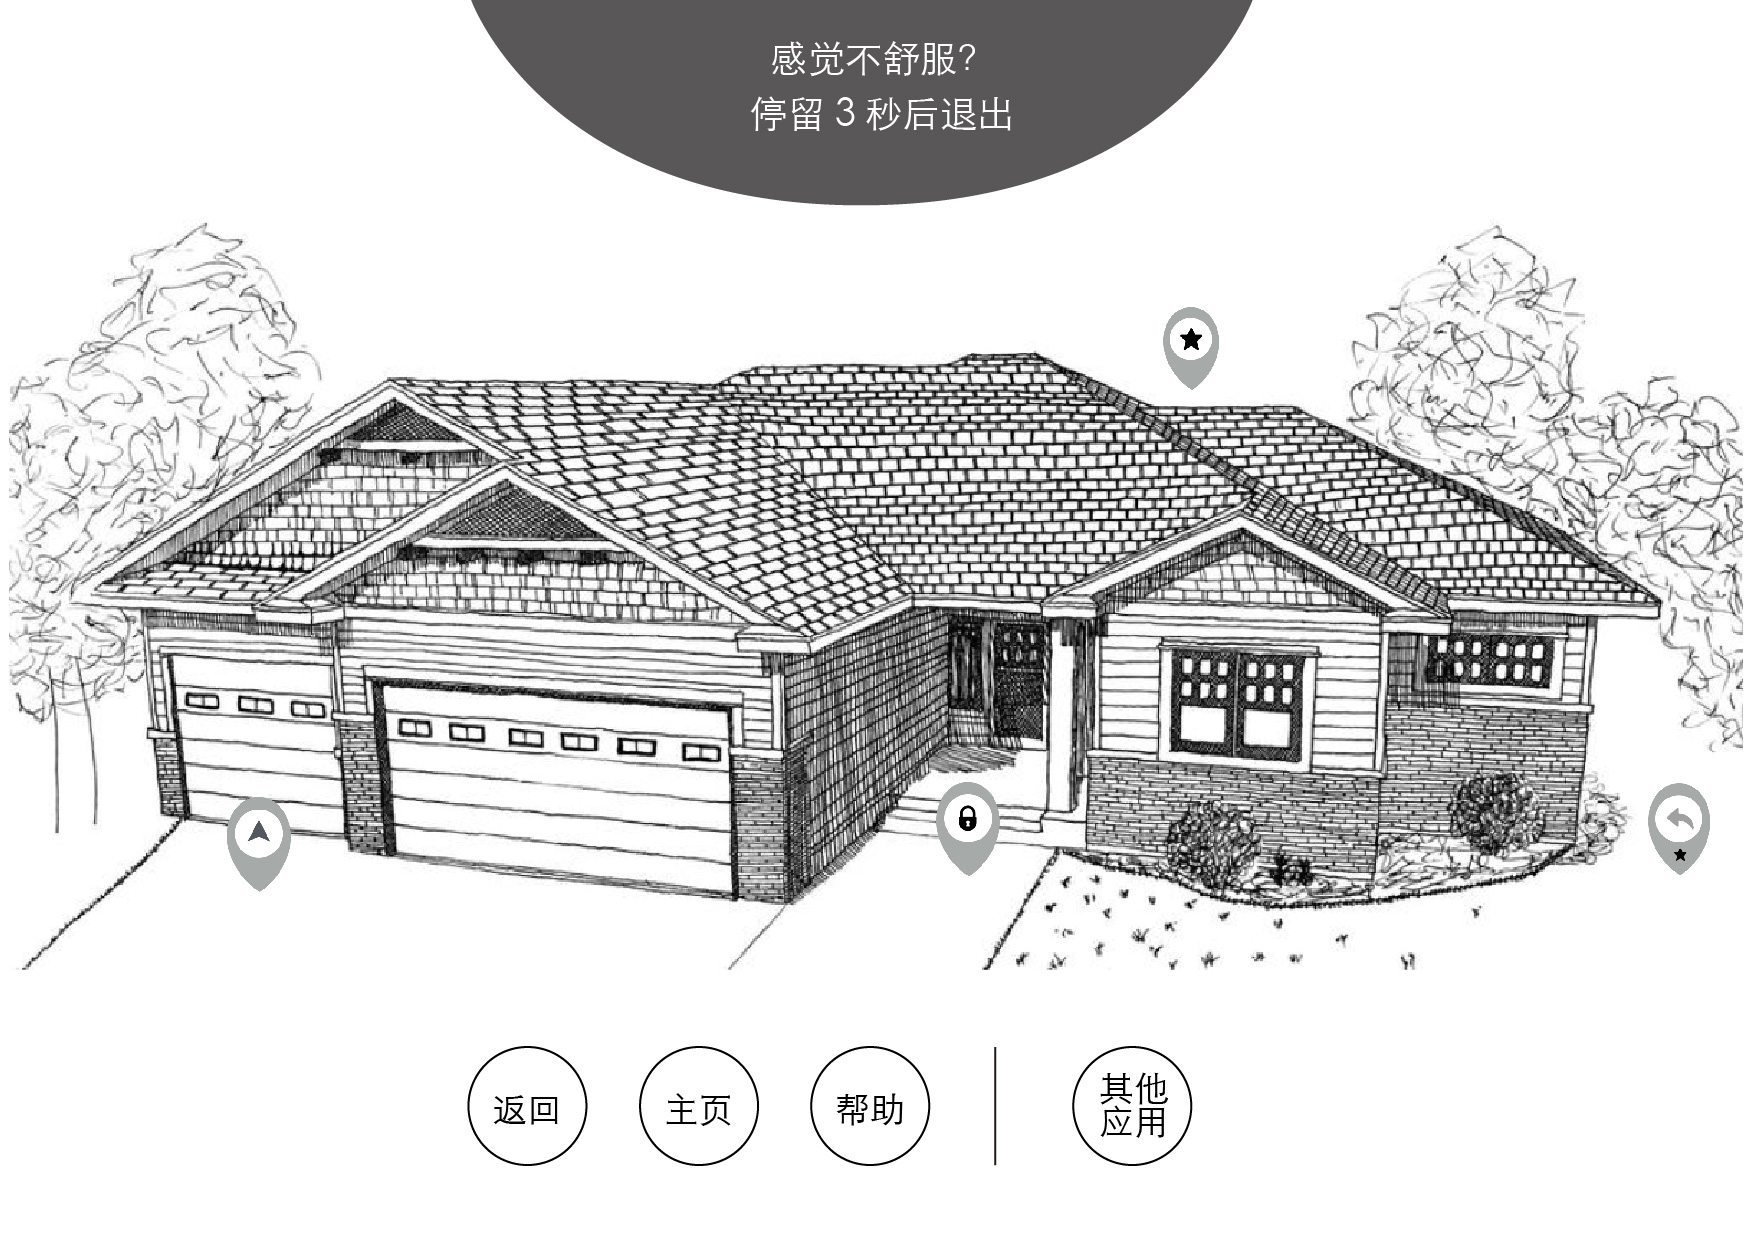
\includegraphics[width=.5\textwidth]{design/d-08}
}
\caption{漫游界面设计}
\label{fig:scenery}
\end{figure}

\subsection{功能界面设计}

语音搜索界面如图\ref{fig:d-04}。

\begin{figure}[htp]
\centering
\fbox{
  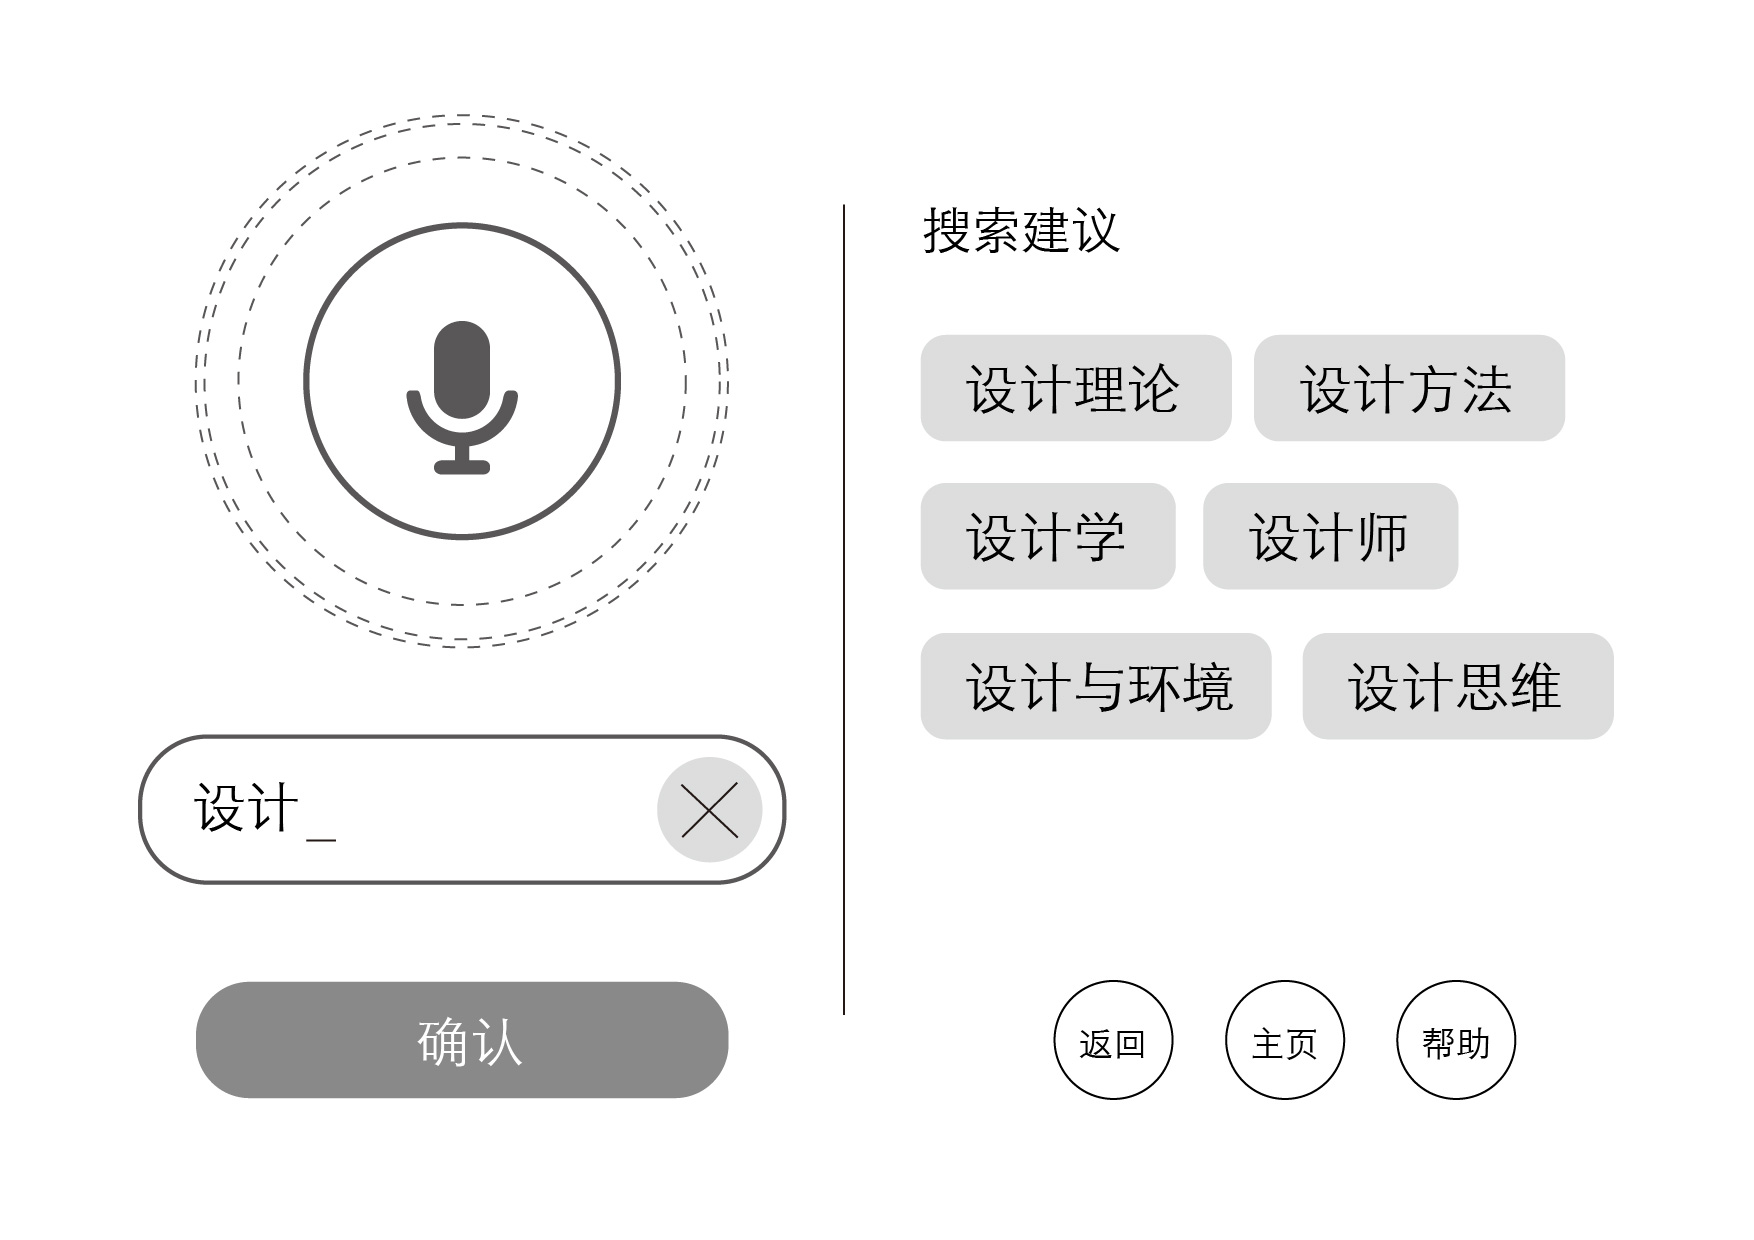
\includegraphics[width=.5\textwidth]{design/d-04}
}
\caption{语音搜索界面}
\label{fig:d-04}
\end{figure}

设置界面如图\ref{fig:d-05}。

\begin{figure}[htp]
\centering
\fbox{
  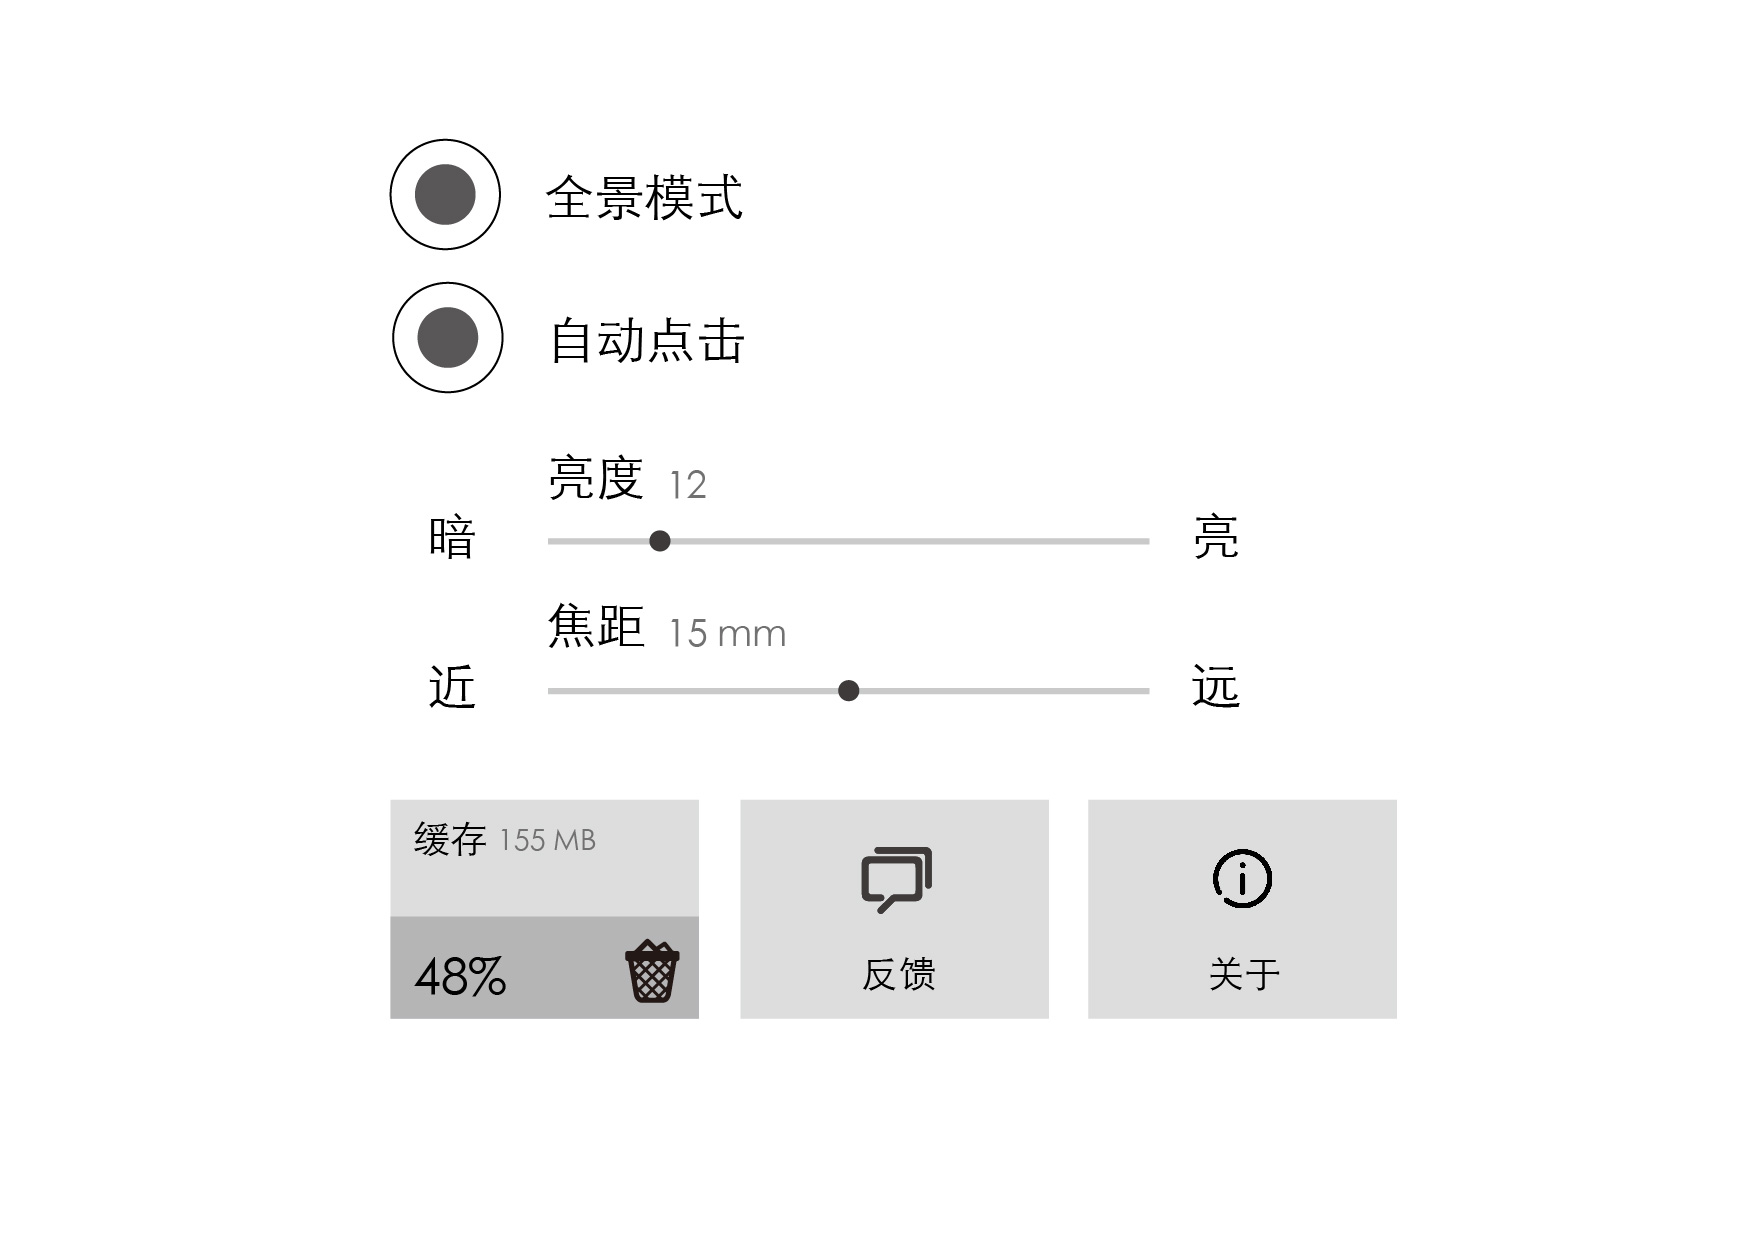
\includegraphics[width=.5\textwidth]{design/d-05}
}
\caption{设置界面}
\label{fig:d-05}
\end{figure}

\subsection{操作方式设计}

前翻和后翻功能是类似书本翻页的功能,可以被用户较为轻松地理解为场景的切换功能,但场景的切换一般为通过触发场景内特定指向箭头,不宜于用户直观寻找,故设置前翻或后翻控件,当视线短时二次进入时可触发切换场景(类似于翻页)的操作,其设计借鉴于移动端场景漫游中上下拖动切换场景的操作\endnote{赵晓倩,王晨升,陈亮,王冬冬. 移动端三维界面两种交互方式的比较研究[J]. 产业与科技论坛,2012,(15):80-81.}。因全景漫游中上下空间被导航栏使用,左右摆头可能为更适合全景漫游切换场景的方式,同时考虑操作中的容错率,快速摆头至指定区域两次可视为一次完整的头部动作,从而触发切换场景的操作。
操作方式示意如图\ref{fig:d-09}。

\begin{figure}[htp]
\centering
\fbox{
  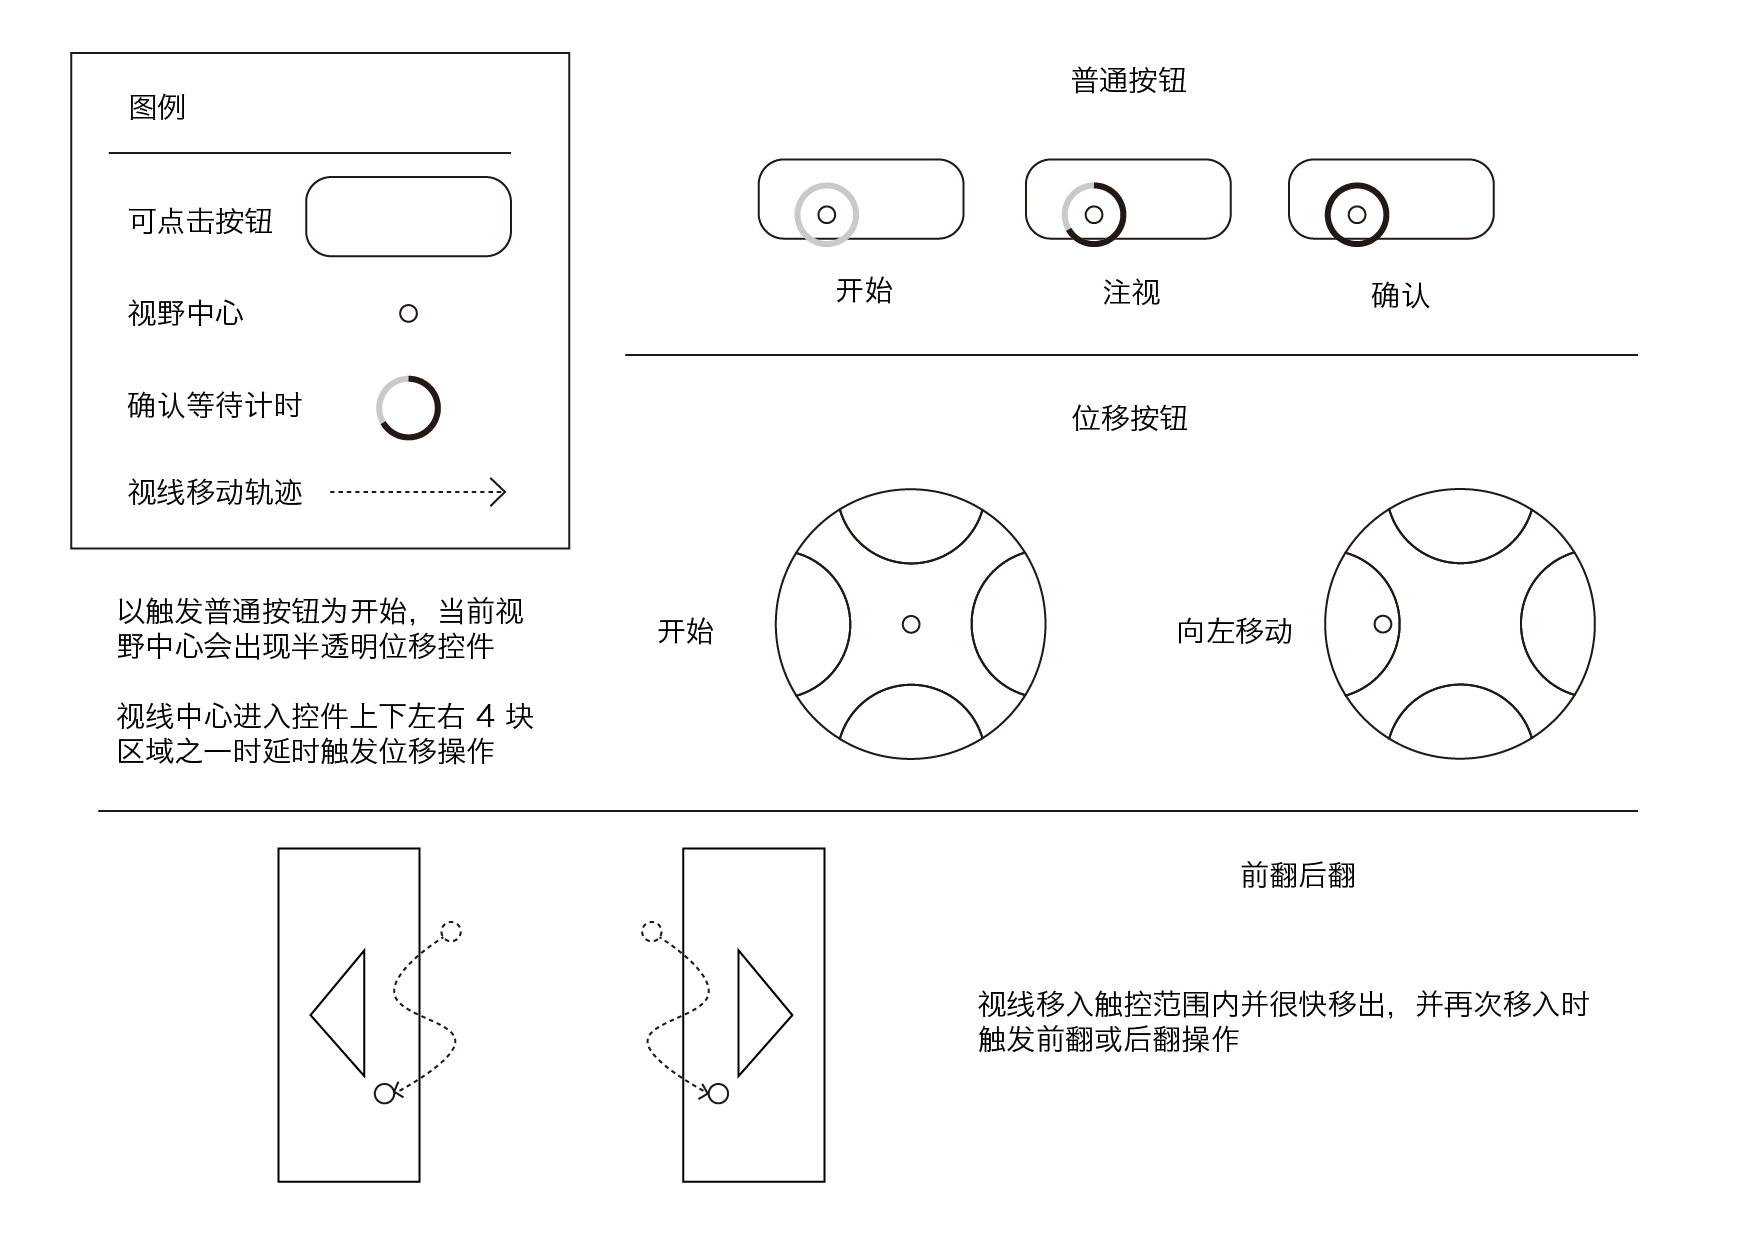
\includegraphics[width=.9\textwidth]{design/d-09}
}
\caption{操作方式示意}
\label{fig:d-09}
\end{figure}